%!TEX root = ../thesis.tex

\cleardoublepage
\chapter{Evaluation}
\label{cha:evaluation}

This chapter reviews how the approach from the previous chapter was tested, and discusses the observed results. This chapter will explain the setup of the testbed, as well as the motivation behind the types of tests which were performed. Finally a discussion of the results and their origins will take place.


\section{Approach to Evaluating Performance}

In order to evaluate the success of the proposed approach a multipath scenario with four links will be emulated and investigated. Each test will consist of two WAN connectors, and the four emulated links going between them. The characteristics of the links will be changed during the tests, each time with respect to different properties: latency, packet loss, and jitter. The evaluations will be performed on a testbed consisted of four seperate host servers. Two of these servers will act as the originating and terminating WAN Connectors. One server will generate and measure traffic, in between the two WAn Connectors, a server will act as the link emulator. This architecture is shown in figure \ref{fig:testbed}

\begin{figure}[h]
    \centering
        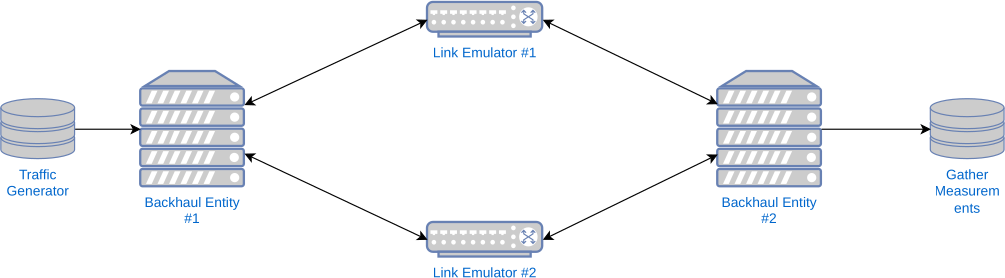
\includegraphics[width=0.66\textwidth]{fig/testbed.png}
        \caption{Testbed Setup}
        \label{fig:testbed}
\end{figure}

In figure \ref{fig:testbed}, the links between the servers are 10 GB ethernet cables. The hosts are connected as is shown. In the "traffic generator and measurer" two linux namespaces are used to separate the traffic generation and the measurement. The packets generated in one namespace are routed via the ethernet connection to the next host (the terminating or "edge" WAN Connector), because of the linux namespace they are not aware that their destination is technically the same host. The packets are then are backhauled by the WAN Connector over the emulated links in the next host, and via the terminating WAN Connector, back to the original host, but now in the "measurer" namespace.

The link emulation is done using the tc subsystem. First a root Heirarchical Token Bucket qdisc is established on the "downlink" and "uplink" interfaces (the ethernet cables between the WAN Connectors). In this case, the link emulation is performed before the outoing packet is queued on the ethernet cable, so that is also where the qdisc is placed. Secondly, the qdisc is given children classes, one class per link. This allows one to establish bandwidth caps for each emulated interface. Within these HTB classes the root qdisc is a netem qdisc. These allow the installation of link characteristics such as latency, packet loss, and jitter.

%In all of these scenarios the same traffic flows will be replayed. This traffic will contain different types of flows, with different QoS requirements. Before a new flow is started, the flow's requirements are sent to the WAN connector and it is either accepted or rejected. During the traffic replay, the delay, jitter, and reliability will be measured.

%All of these tests can be performed on the same testbed which will be set up as is shown in Figure \ref{fig:testbed}. The testbed architecture features a traffic generator, two WAN connectors, with a link emulator between them, and a measurement module to analyze performance. In practice the traffic generator and the test bench will be co-located on the same machine. The link emulator, and the WAN connectors are separate hosts, all interconnected over ethernet. The link emulation is done using the linux kernel's traffic control subsytem (TC). TC offers a network emulator (netem) queuing discipline (qdisc), which is able to emulate various link characteristics including delay, jitter, packet loss and packet re-ordering. Furthermore by combining the netem qdisc with a rate limiter, such as the Heirarchical Token Bucket (HTB) qdisc, a link can have its bandwidth limited. This allows one to emulate links with different latency, reliability and jitter, and with different maximum bandwidths.

In order to make the emulation more realistic, the netem qdiscs will periodically be adjusted, this allows one to degrade or improve links over time, for example by increasing the latency or packet loss in frequent intervals, up to a large value. It also more closely mimics the real-life behavior of WAN connections, which do experience changes in their characteristics over time.

For the purposes of evaluating the WAN connector, three series of experiments will be performed to isolate and investigate it's link switching capabilities. First, purely latency based link selection will be investigated- a flow will be defined with specific latency requirements and then the emulated links will have their latency repeatedly changed. The same will be done once with packet loss and with jitter. In each of these scenarios the other two parameters will be held constant, so that the WAN Connector can be judged based on its ability to meet one of the latency, jitter, or packet loss requirements, without the other two requirements interfering. In order to simulate realistic scenarios these experiments will also be repeated once with background traffic which aims to saturate the link's capabilities.

The data for the emulation used in all of these scenarios was obtained using the Satellite Constellation Network Emulator (SCNE) \footnote{https://connectivity.esa.int/projects/scne} from the European Space Agency. The default scenario is 24 hours long and consists of 288 satellites, 10 gateways (GW), and 50 user terminals (UT). The reason this data is used is because LEO satellite links are expected to be the most common type of backhaul link for geographically distributed 5G Campus Network deployments. Furthermore, since LEO satellite connections are exceptionally more volatile than "regular" links \cite{deutschmann2022broadband} \cite{ma2023network}. By choosing to emulate more volatile links in the testbed, the WAN Connector experiences a more difficult test, and one can be assured that the real life performance in "normal" scenarios, is highly unlikely to be worse.

Since the WAN Connector is defined to work on at most four outgoing links, each investigated scenario will feature four links. These links will all be based on data from the SCNE emulation.

\subsection{Accuracy of the Emulation}

To make sure that the testbed emulation also matches the values from the SCNE, a brief comparison was done, where the testbed's latencies were compared with those recorded in the SCNE. 

Figure \ref{fig:sim_vs_em} shows the comparison between the data observed in the testbed, and the SCNE. The testbed data in the graphic is measured by the packet flows running over the individual links. The emulation data comes from the values recorded during withh the SCNE. Since the testbed data is collected at a rate of 100 packets per second, but runs at 10 times the speed of the SCNE emulation, there are 10 times as many data points. This explains why the testbed data appears blurrier.

\begin{figure}
  \centering
  \begin{tabular}{@{}c@{}}
    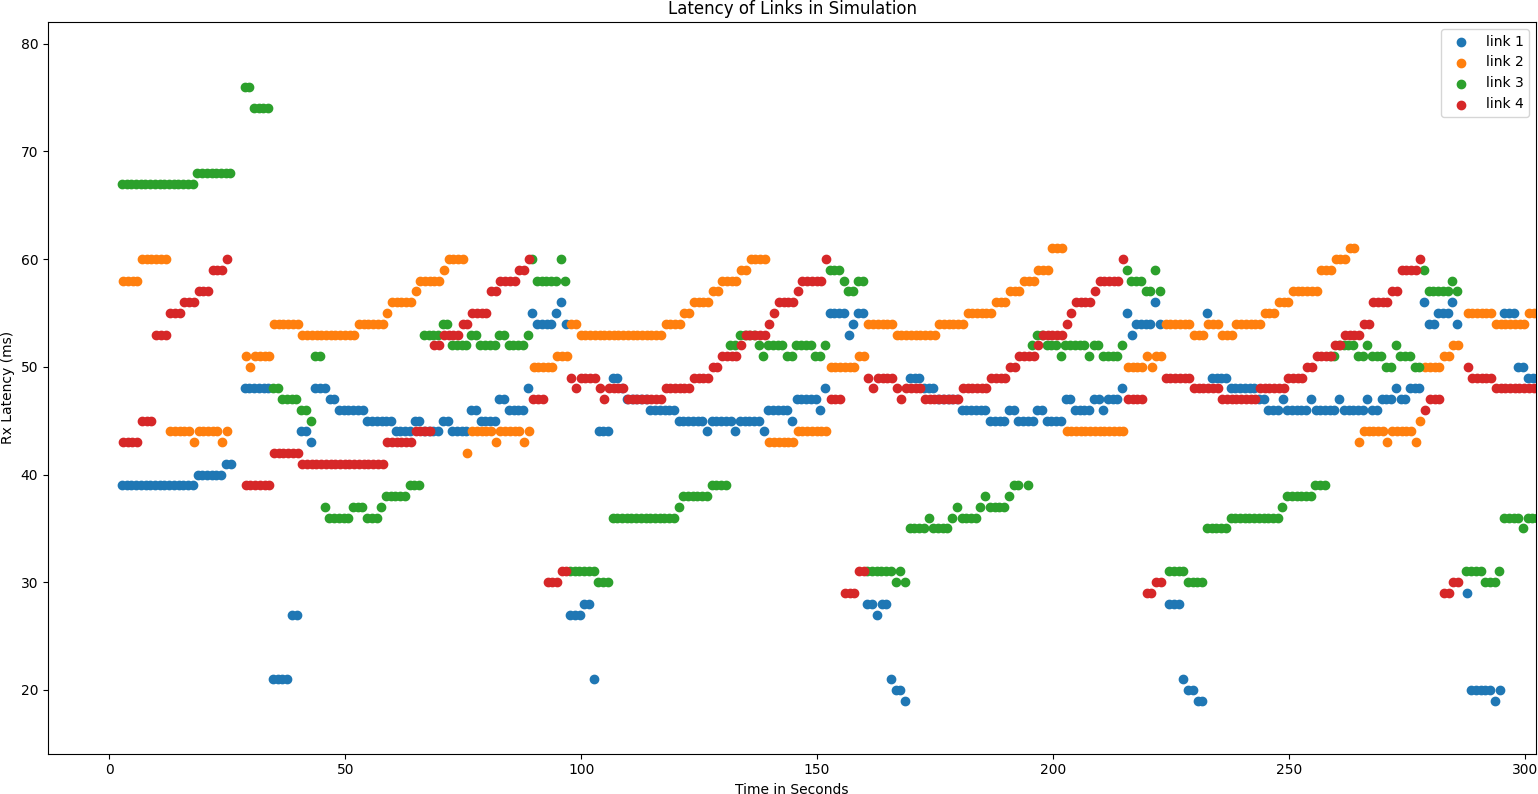
\includegraphics[width=\linewidth]{fig/simulated_latencies.png} \\[\abovecaptionskip]
    \small (a) Latencies Recorded in SCNE
  \end{tabular}

  \vspace{\floatsep}

  \begin{tabular}{@{}c@{}}
    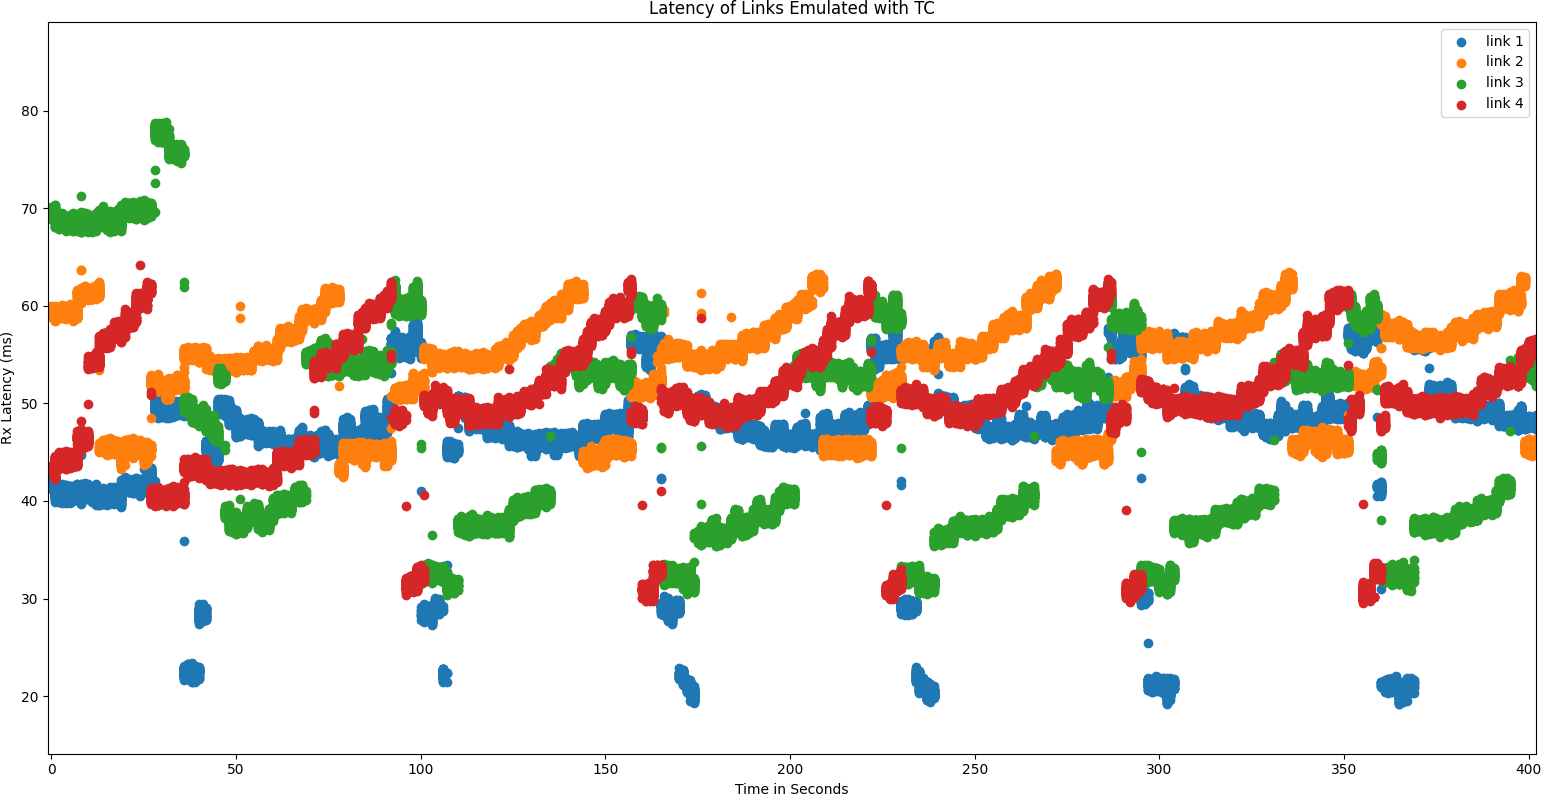
\includegraphics[width=\linewidth]{fig/emulated_latencies.png} \\[\abovecaptionskip]
    \small (b) Emulated Latencies Measured in the Testbed
  \end{tabular}

  \caption{Comparison of the Emulators Latencies and the Testbed}\label{fig:sim_vs_em}
\end{figure}

As can be seen in the figure \ref{fis:sim_vs_em}, the latencies recorded on the testbed closely match those from the SCNE, which it was seeking to replicate.

\section{Latency Based Path Switching}

First is the scenario investigating latency. During the emulation, the simulation data is used to adjust the tc netem qdisc on the "link emulator" machine periodically. Because the SCNE simulator provides latency data over a 24 hour period, in 10 second intervals, the simulation data is "sped up". That is the emulation is changed each second, based on the next datapoint from the simulation. This means the 24 hour window can be run over a 2 hours test. Since real links are usually steadier and less volatile than the sped up emulation one can expect results in a real situation to be better.

In the experiment 100 packets are sent per second across each link, as well as 100 packets per second from the traffic generator, through the WAN Connector. This is done to have a comparison between the performance of the WAN Connector and the baseline performance level, which would be the best performing link. In any scenario the minimum acceptable performance of a path switching application would be to provide a better performance than the best single link. Otherwise it would be better to just select the best link, and not use the application at all.


\subsection{Performance Compared to Single Links}

For the experiment a flow is defined in the WAN Connector with a minimum round trip time (RTT) of 56 milliseconds. This value is chosen because it is the mean of the mean values of the latencies of the four links from the emulation. For the evaluation of the latency based path switching a single flow matching the definition stored in the WAN Connector is backhauled through the WAN Connector at a rate of 100 packets per second. In order to serve as a comparison, identical 100 packet per second flows are sent across the four other links. Finally their latencies are compared, and the latencies measured by the four links are used to calculate the Oracle approach.

The graphics \ref{fig:latency_cdf1} and \ref{fig:latency_cdf1_super_zoomed_in} show a cumulative distribution of the different latencies experienced by the packet flows running over the individual links and the WAN Connector, as well as the performance of the Oracle approach. The Oracle results are purely theoretical. For each packet, it is able to select the best link to forward on, based on that links future characteristics. This approach is calculated by comparing each packet sent by the WAN Connector with the latency that packet \textit{would} experience on any of the other links, and if the latency of the WAN Connector's link would be greater than the minimum value (56 ms), selecting a different link (if one exits) with a lower latency. Since it always picks an optimal path, the Oracle approach provides an upper bound on the best possible performance. In practice it is not possible because it has knowledge of the future, but nonetheless it acts as a very valuable comparison.

\begin{figure}[h]
    \centering
        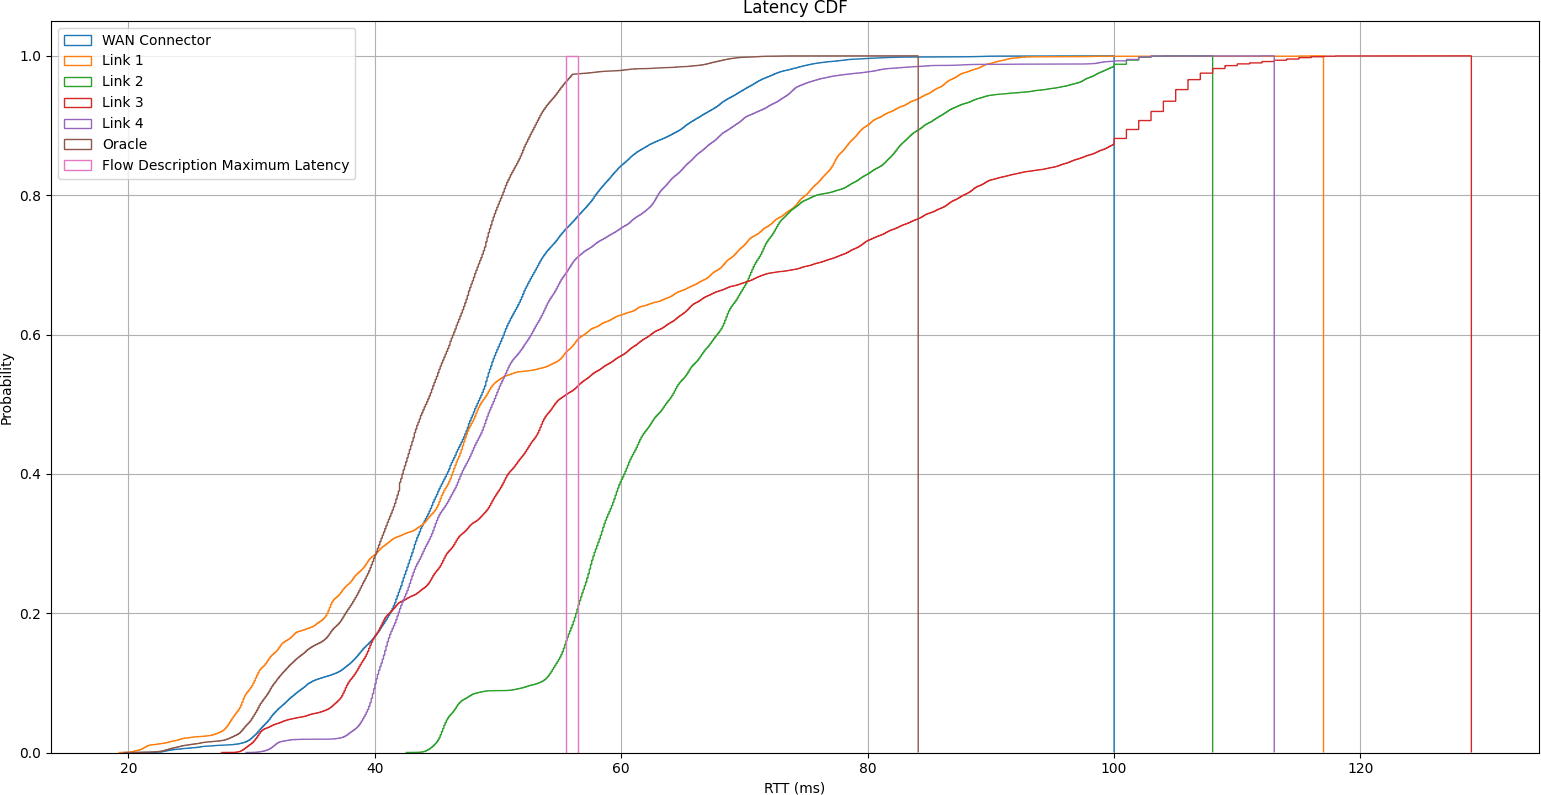
\includegraphics[height=0.8\textwidth,width=\textwidth]{fig/latency_cdf1.png}
        \caption{Cumulative Distribution of the Latencies}
        \label{fig:latency_cdf1}
\end{figure}

\begin{figure}[h]
    \centering
        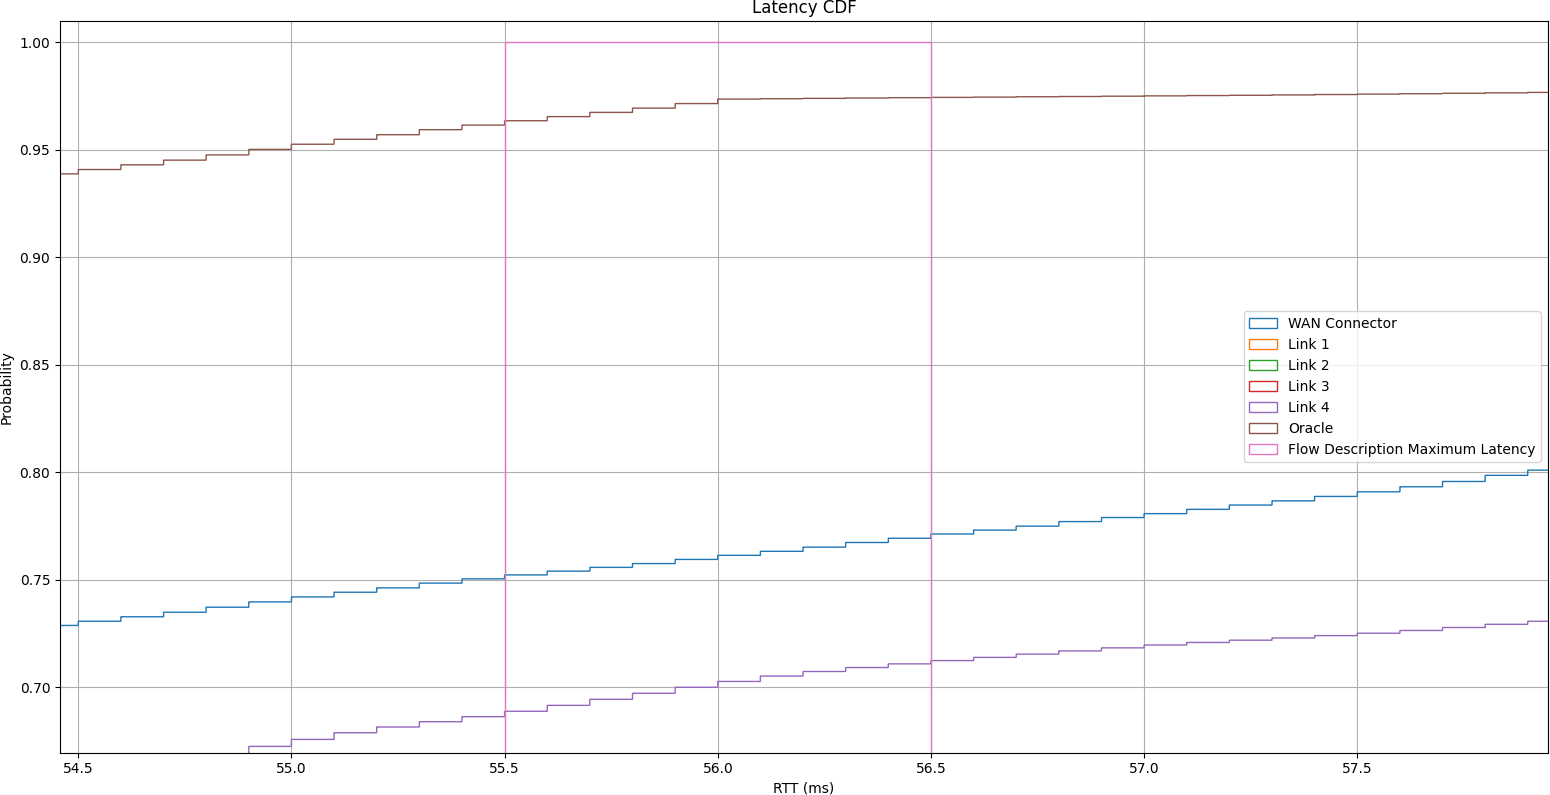
\includegraphics[height=0.66\textwidth,width=\textwidth]{fig/latency_cdf1_super_zoomed_in.png}
        \caption{Closeup of the Latency CDF}
        \label{fig:latency_cdf1_super_zoomed_in}
\end{figure}

The CDF shown in figure \ref{fig:latency_cdf1} and zoomed in on in figure \ref{fig:latency_cdf1_super_zoomed_in} tracks the probability that the flow experiences a latency less than or equal to the latency value on the y axis. The pink bar labelled "Flow Description Maximum Latency" is set at 56 milliseconds and represents latency bound for the flow being measured, which was communicated to the WAN Connector.


The results in the figures show that the WAN Connector is able to achieve a superior performance to any of the individual links on their own. This was the baseline requirement and it is important that it is able to achieve this. However the performance does not significantly improve on the next best link, which is is able to achieve the maximum allowed latency 72\% of the time, while the WAN Connector does so 77.5\% of the time. The Oracle approach shows that in theory one could, at best, have maintained the minimum latency required by the flow in 95\% of the cases. This means the WAN Connector's performance is only 80\% optimal.


\subsection{Latency Performance Under Load and the Importance of Traffic Shaping}

During this experiment, the same 100 packet per second flow from before is repeated, but background traffic is added. An iperf3 test is run across the WAN Connector at the same time as the latency critical flow, and the background traffic is given the same latency requirements, so that the WAN Connector always schedules both flows to the same link. This ensures that whatever link is being used will be saturated. Latency performance during congestion and close to congested scenarios is a crucial element of a deterministic backhaul solution. The WAN Connector's control plane only makes decision about which link to forward on- it does not perform load balancing or prioritization. The data plane does not do this either, it implements a purely First In First Out (FIFO) approach to packet queuing. This is done because the burden of implementing an appropriate packet shaper, in addition to the other multipath calculations, is too significant for the purposes of this thesis, and because very powerful traffic shaping implementations, which are easy to integrate into this solution, already exist.

\begin{figure}[h]
    \centering
        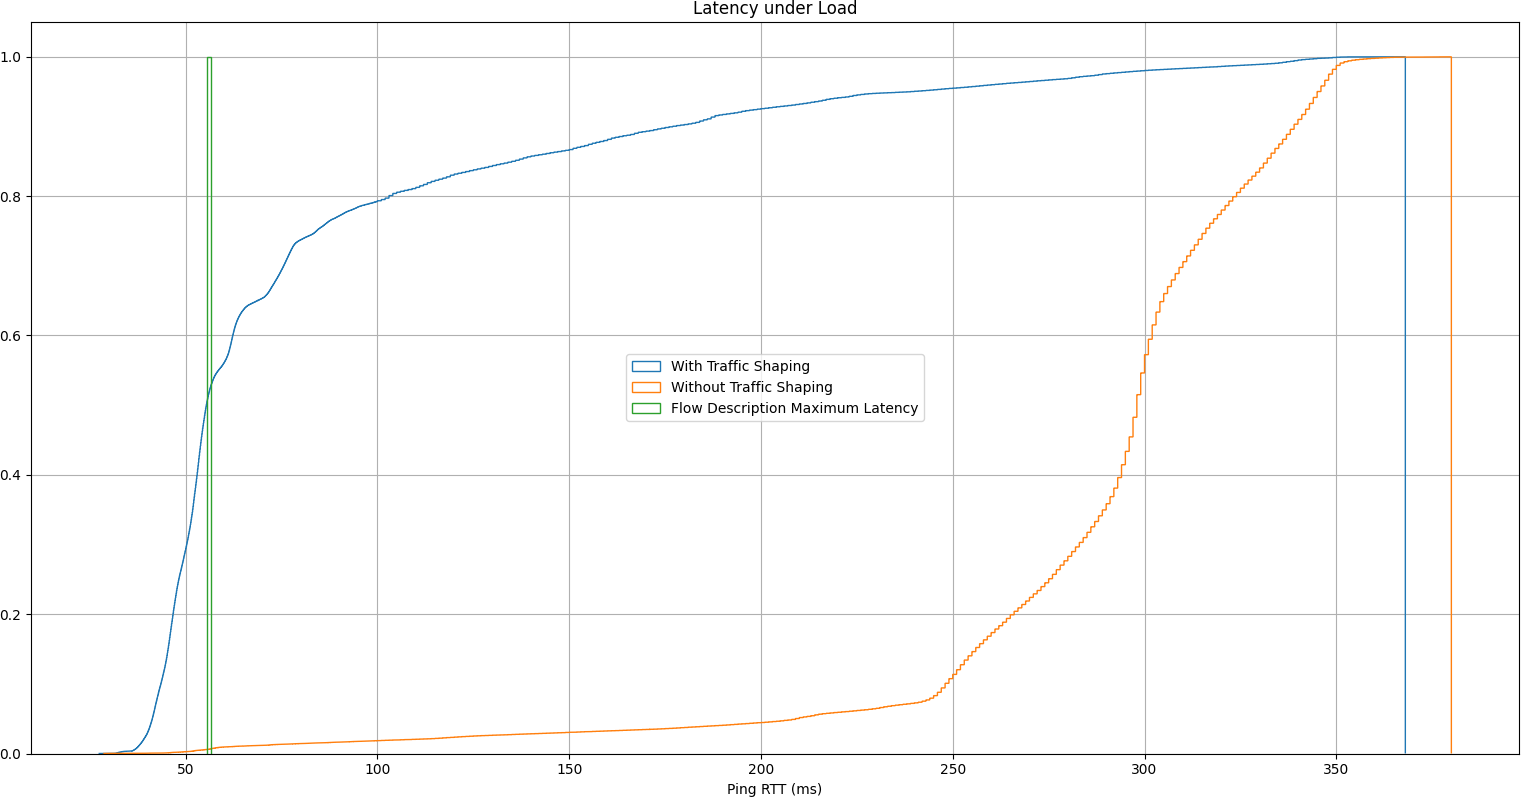
\includegraphics[height=0.66\textwidth,width=\textwidth]{fig/rrul_cdf.png}
        \caption{Latency with Background Traffic}
        \label{fig:rrul_cdf}
\end{figure}

The figure \ref{fig:rrul_cdf} neatly demonstrates why traffic shaping is an essential element of any deterministic network. In the case in which there is no traffic shaper the latency critical flow experiences significant additional latency due to the network being overloaded. The TCP algorithm fills the link's capacity, and the latency critical packets spend too much time buffering and arrive late. It should be noted that the WAN Connector's performance with the traffic shaper is worse than in the previous scenario, where there was no background traffic, and only 50\% of the packets are under the required latency of the critical flow. However the approach without the traffic shaping is at just 1\%.

\section{Reliability Based Path Switching}

In the next scenario, to analyze the ability of the WAN Connector to achieve the required reliability of a given flow, the same test flows from before are run over the WAN Connector and the four outgoing links. However this time instead of varying the latency, the packet loss ratio of the link is changed. The SCNE emulation's data is used for the testbed once again. However since the emulation does not provide packet loss on a per second basis, the latencies of all the different links in the simulation are used. For the emulation, these 51 values are looped over in 10 second increments. Each link is given a shuffled set of these 51 values. This means that the cumulative value of the packet loss experienced by all of the links is the same (2\%), but the instantaneous values will differ. To appropriately analyze this scenario the flow being backhauled over the WAN Connector is given a reliability threshold of 0.1\% this is because in this scenario, where the existing links all provide an average of 2\% reliability, it becomes necessary to duplicate at some points, in order to achieve the required reliability. Afterward, the experiment is repeated under load, like in the latency scenario, where the test flows across the links themselves are not run, and a second iperf3 flow is run across the WAN Connector in order to saturate the link. Like before, this second flow is given the exact same requirements as the test flow, in order to ensure that they are always running across the same link.

 The results of this experiment are shown in figure \ref{fig:loss_bars1}. The packet loss recorded by each of the flows over the period of the experiment is plotted in a bar graph, as well as the theoretical packet loss which would have been experienced by the Oracle approach.

\begin{figure}[h]
    \centering
        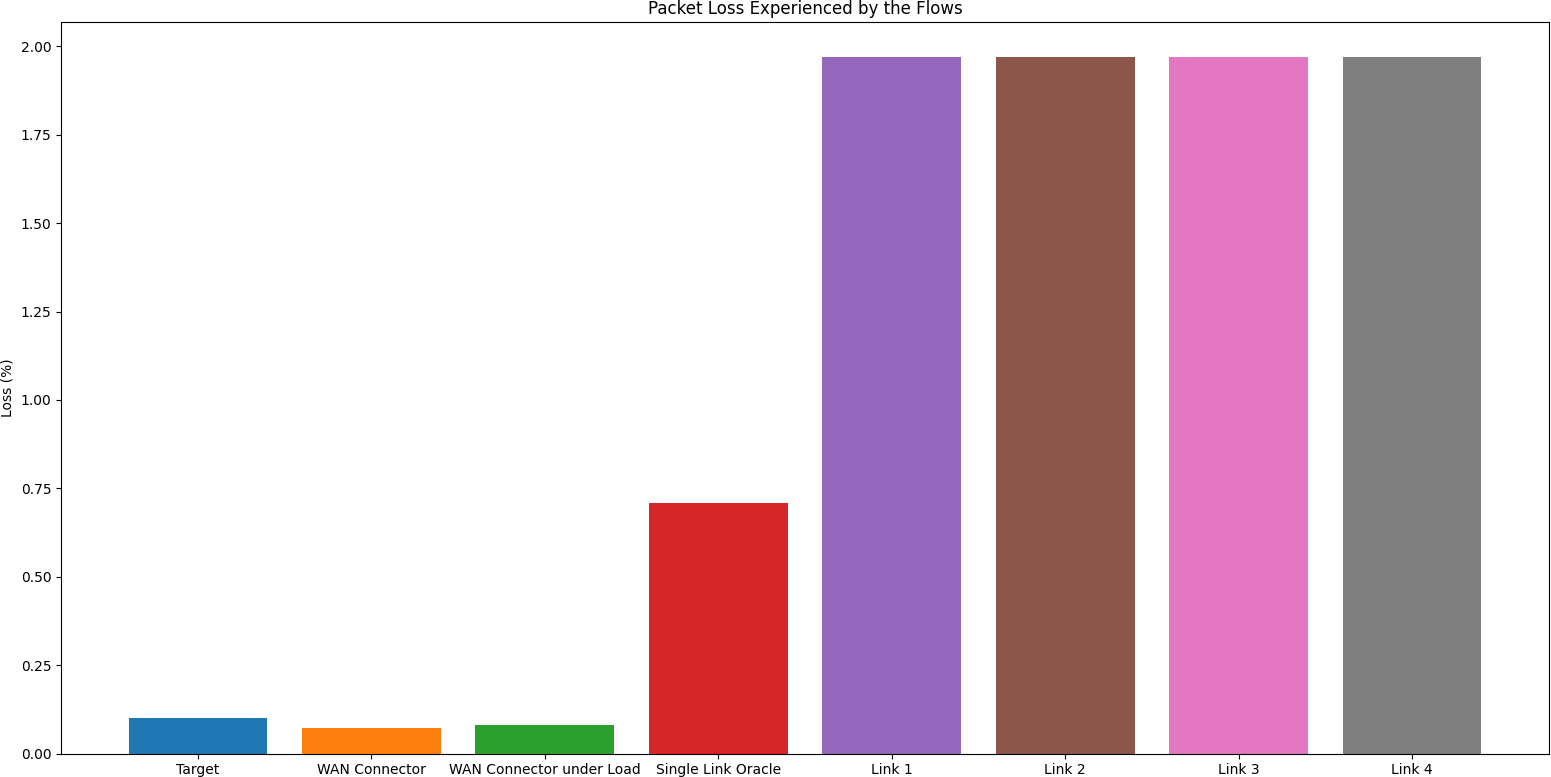
\includegraphics[height=0.66\textwidth,width=\textwidth]{fig/loss_bars1.png}
        \caption{Reliability}
        \label{fig:loss_bars1}
\end{figure}

For the analysis of the performance this time the Oracle approach is defined as choosing, before forwarding any packet, the link with the lowest packet loss ratio. But, crucially, the Oracle is not allowed to duplicate flows across different links. This explains why in figure \ref{fig:loss_bars1} the Oracle is outperformed by the WAN Connector. Indeed, as the graphic shows, it is not possible to achieve the critical flow's required reliability with any of the available links, nor with the Oracle approach. But the WAN Connector is able to achieve it. This speaks to the potency of the flow duplication approach, which is made possible in the optimization equation used to decided on which flows to forward.

\subsection{Impact on Throughput}


\begin{figure}[h]
    \centering
        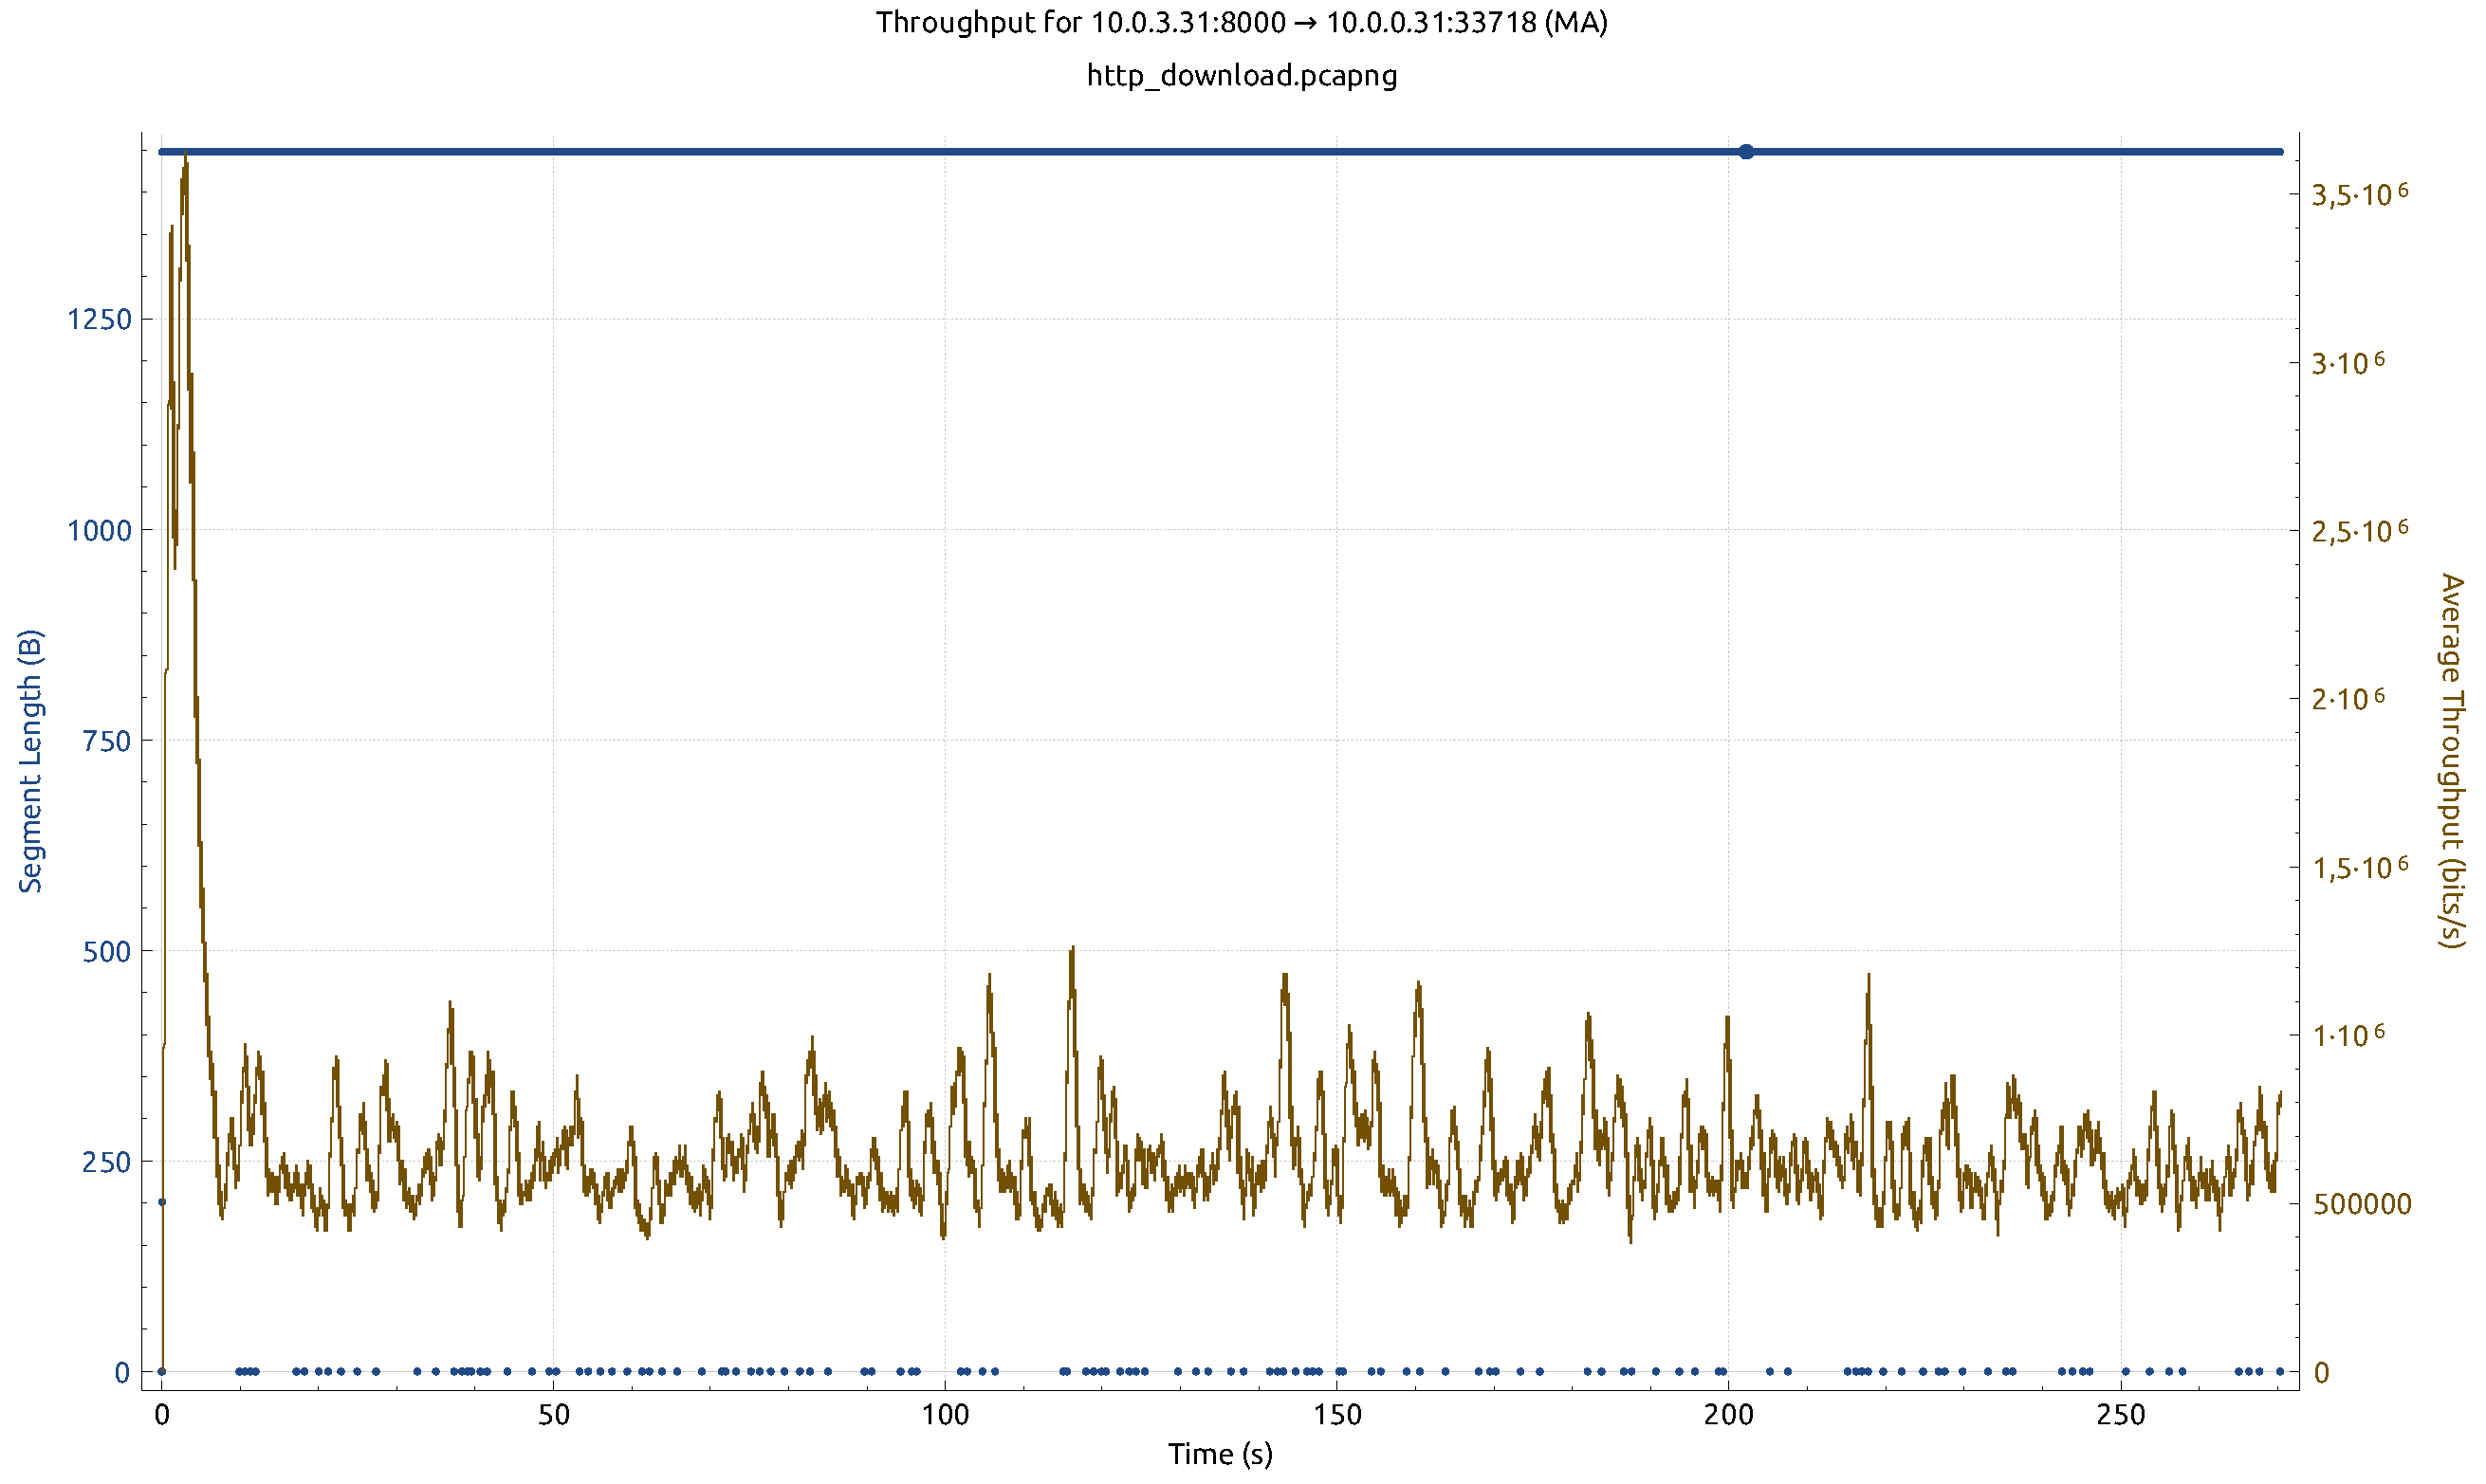
\includegraphics[height=0.66\textwidth,width=\textwidth]{fig/tcp_throughput.pdf}
        \caption{Throughput of a Duplicated Flow}
        \label{fig:dup_tcp}
\end{figure}

One of the unfortunate impacts of packet duplication is that it reduces the available bandwidth. It represents a waste of up to 50\% of the available resources, in the worst case, where every flow must be duplicated. Additionally, since flows which are being duplicated need to be re-ordered, this means that the FIFO approach for packets cannot be used and instead the packets must pass through a Packet Ordering and Elimination Function (POEF). When a packet arrives out of order the POEF starts to incur significant additional overhead because it must store all packets until the missing packet arrives, or a point is reached at which the stored packets must be dequeued. This point is either the point at which the packets expire, or the queue of out of order packets becomes full. Beyond this, the storing and eventual mass de-queuing of out of order packets can also interfere with the TCP algorithm- thus leading to reduced throughput.

These two effects - the POEF overhead and it's effects on TCP- lead to a very heavily reduced throughput, as can be seen in figure \ref{fig:dup:tcp}. The graph in the figure shows the throughput experienced by a routine TCP download, running over the WAN Connector, and experiencing replication, as well as the segment length of the TCP stream. As can be seen in the graph, the throughput is very low, and is not able to saturate the link's bandwidth despite being the only flow running at the time.

\section{Jitter Based Path Switching}

\begin{figure}[h]
    \centering
        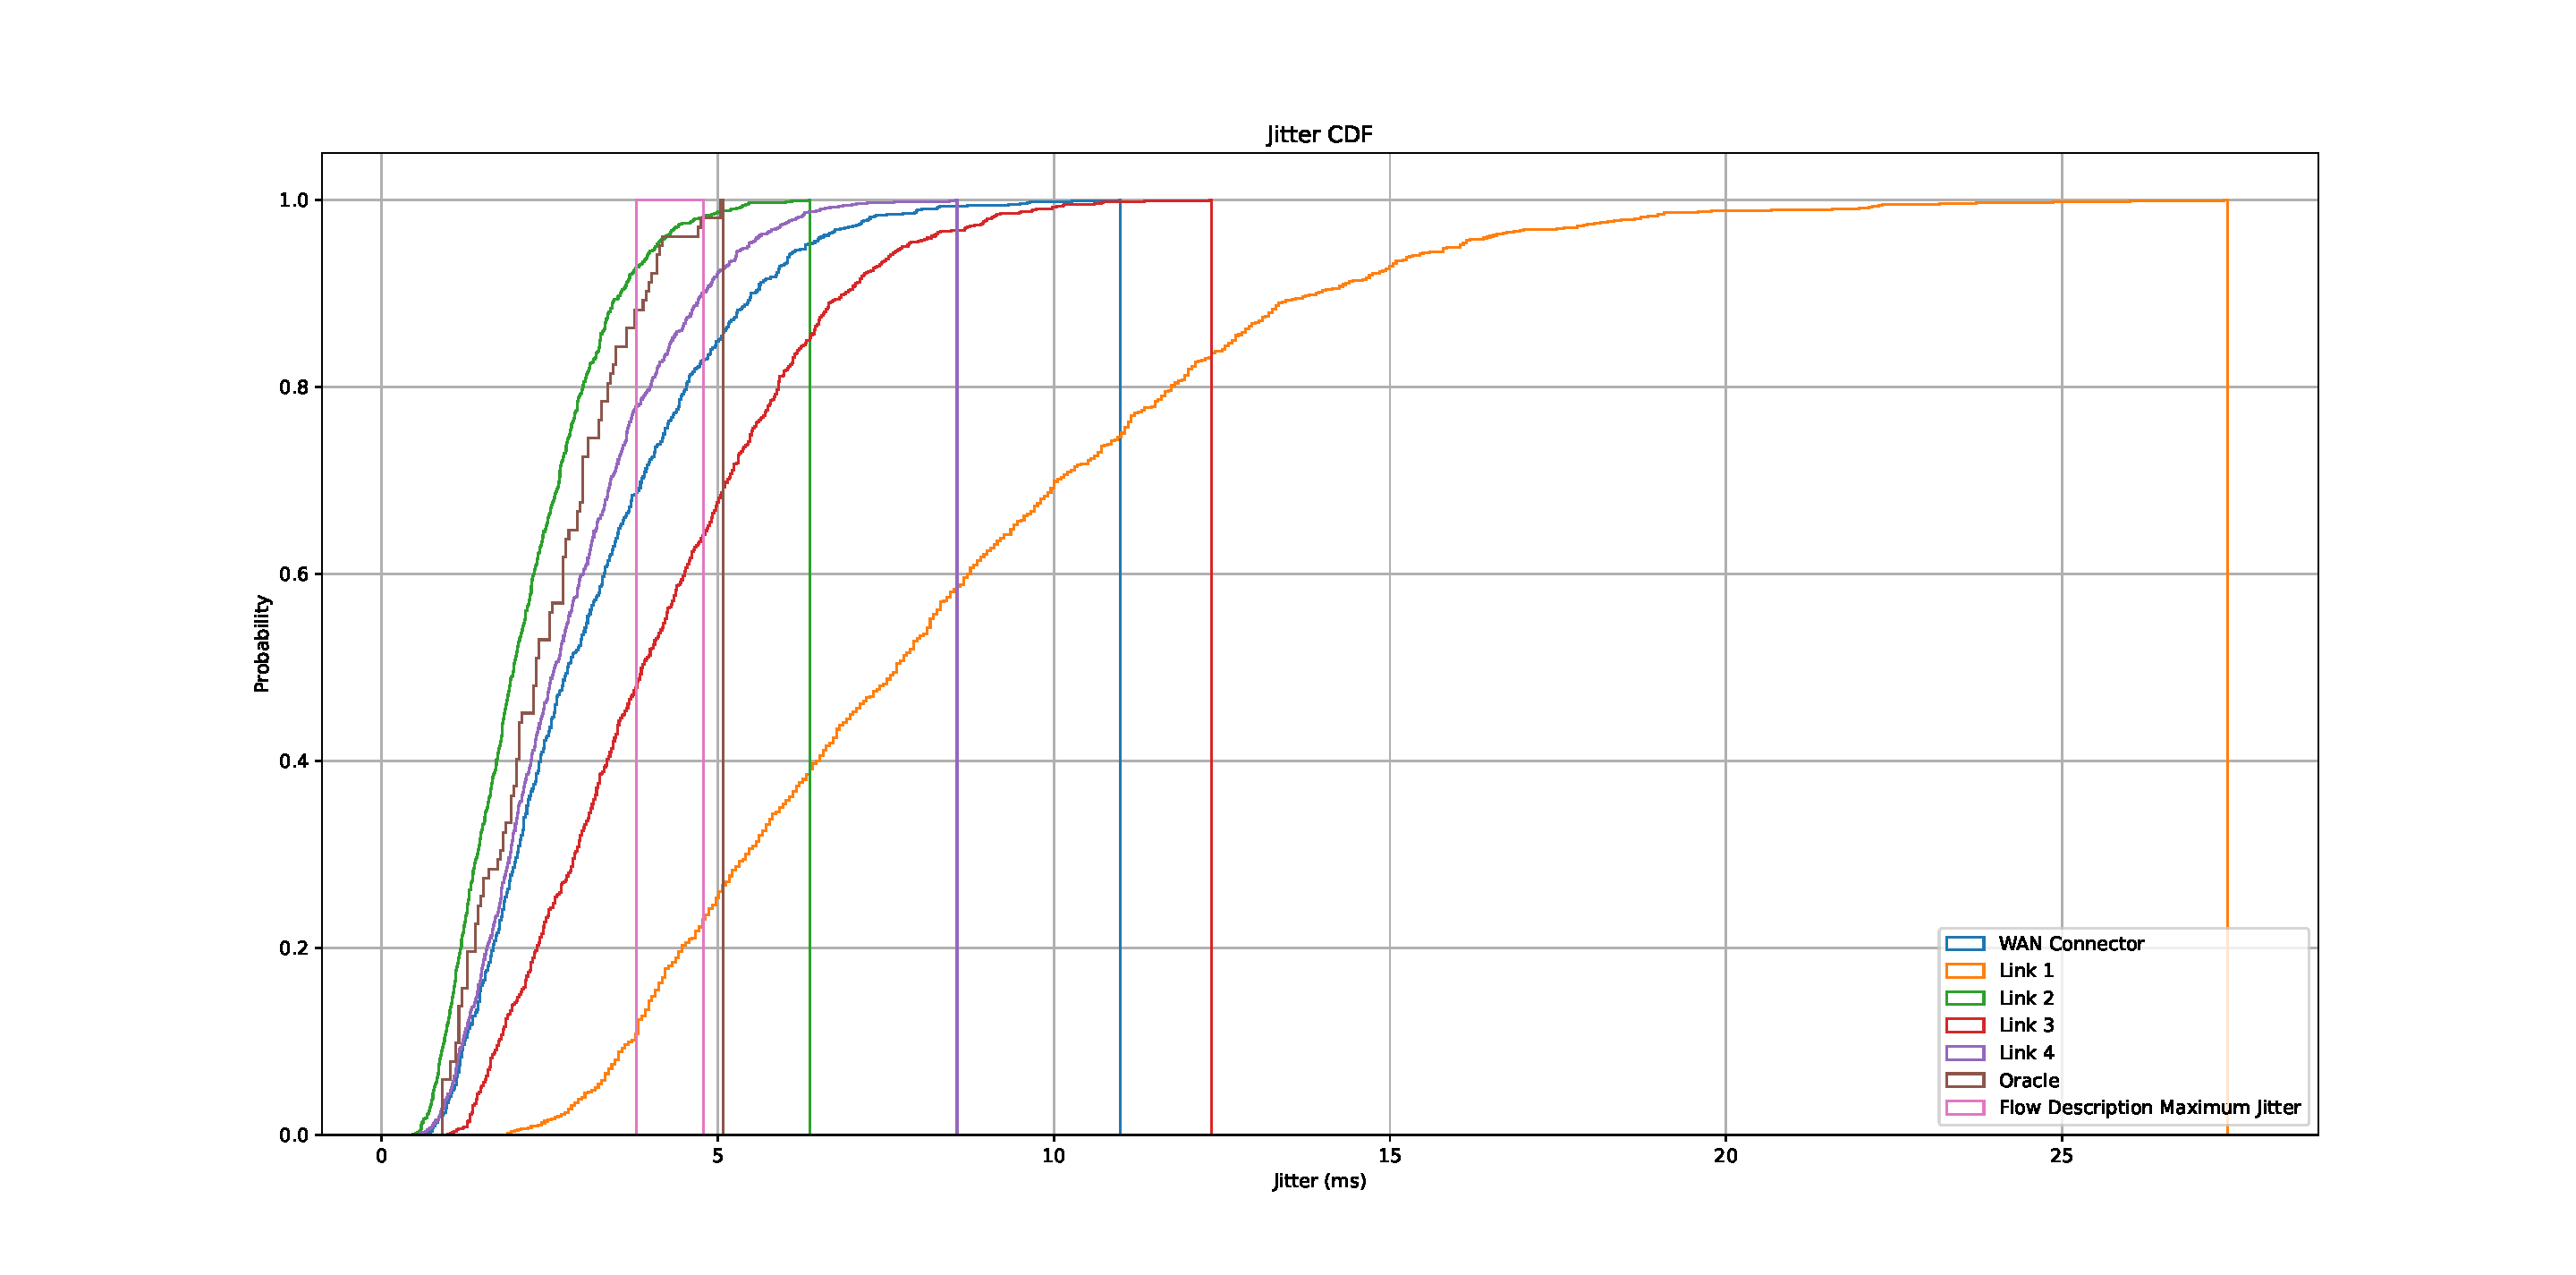
\includegraphics[height=0.66\textwidth,width=\textwidth]{fig/jitter_cdf.pdf}
        \caption{Performance of Jitter Based Path Switching}
        \label{fig:jitter_cdf}
\end{figure}

For the final analysis, the jitter must be investigated. For this purpose the simulation data was once again adapted. This time the standard deviation of the latency experienced was calculated for each of the 102 connections in the simulation. Then these standard deviations were scaled down by diving them by one, two, three, and four, respectively, in order to acquire four different set of jitter characteristics. Finally the scaled values were shuffled. This resulted in 4 links with varying jitter characteristics, which suffices for the emulation. Each different jitter value is emulated for 10 seconds on the respective link. During the emulation scenario a UDP iperf3 stream is ran at a rate of 3/4ths of the link's capability for 1000 seconds. iperf3 records jitter each second, and this data is used to then analyse the performance. Since more than half of the link capacity is being used by the flows being sent on the links (and not through the WAN Connector), the WAN Connector cannot be tested at the same time. Thus, to test the WAN Connector the emulation is repeated but with the flow only being sent over the WAN Connector. Lastly, the Oracle approach is calculated based on the simulation data. The Oracle approach, like before, displays the theoretical optimal performance. It chooses, at each point in time, the link with the lowest jitter. The cumulative distribution of the jitter experienced by the flows is plotted in figure \ref{fig:jitter_cdf}. 

As can be seen from the figure, the WAN Connector gave a very disappointing performance. It displays an inferior performance to two of the links. This means the path switching is actually causing a worse performance. This is most likely down to insufficient statistics causing poor path selection, because jitter statistics can't be gathered about other paths in this single flow scenario. The probe packets which are periodically sent out do not provide enough data points to accurately determine jitter. While they can give a sufficient baseline for latency calculations, as well as helping to determine if a link is dead or alive, their jitter measurements are not likely to provide a strong insight into the true nature of the link's jitter.

A final note about the plot in figure \ref{fig:jitter_cdf}. In the figure the first link actually performs better than the Oracle for most jitter values, before ultimately proving to have the greater maximum jitter values. This occurs because the Oracle is based on the simulation data and not the measurements. Therefore it is likely that the better performing link experienced, for the most part, very low jitter, and thus because there are more data points available than for the Oracle (and because no doubt there was some small amount of luck with the random values used by tc's netem qdisc), the percentage of packets below a certain level of jitter is greater. However ultimately the maximum values experienced by the flow, during those times when the link experiences it's worst jitter, are worse than the Oracle approach's worst cases, as one would expect.


\section{Discussion}

In light of these results one can conclude that the approach presented in the previous chapter is not without its flaws, however the results have also highlighted some of the functional aspects that were important for good performance. For latency based path switching it was able to outperform the other available links and achieve 80\% optimality, and the inclusion of a traffic shaper proved vital for preventing the latency critical flow from experiencing higher buffering times in the presence of a competing flow. For reliability, the WAN Connector showed that it was able to guarantee a critical flow a lower level of packet loss than would have been possible using any single link. Furthermore, it was even able to outperform the single link Oracle, and in a situation where the single link Oracle is unable to provide the required minimum level of packet loss for the desired flow, the WAN Connector was able to deliver the desired reliability. This is a hugely important result because it shows that the WAN Connector can provide greater reliability than even an optimal single link path selection algorithm, via the packet replication. This can enable critical applications to be run in environments where the backhaul options would usually be too unreliable to enable the critical applications.

This section, however, also demonstrates the downside of the packet replication approach, as it greatly reduces the overall throughput. Beyond this, during the jitter experiments, it is seen that the WAN Connector provides a poorer performance than simply using a single link for the entire experiment. This is fundamentally a bad result. The baseline by which any path selection algorithm should be judged is its ability to outperform the individual paths, since it can always select a superior option when one exists. Since the WAN Connector fails in this instance it must be concluded that it cannot provide an overall reduction in jitter for any jitter sensitive applications. The author would suggest, however, that the problem in this respect is not due to the design but rather the implementation. Ultimately there was not enough up to date information about the available links' jitter, so that the path selection algorithm could choose the right one.


%%=========================================
\section{Improvements}

There are several possible improvements that immediately spring to mind. These could be applied both to the actual implementation as well as to the high level design.

\subsubsection{Measuring and Predicting Path Characteristics}
Firstly, the path estimation could be adjusted to not just report previous statistics but also attempt to infer what the path might look like in the near future, for example as a path begins to experience increased latency a predictive algorithm/approach might be able to preemptively move flows off of that path, before their latency requirements are violated. This approach could be based on machine learning or AI, or it could use analytical methods.

Furthermore, it would be prudent to use an exponentially weighted averaging function when calculating a path's current characteristics, based on previous measurements. This would strike a nice balance between re-actively adjusting the predictions based on previous measurements and keeping in mind a path's performance across its entire history.

Also, as the authors in \cite{adaptive} did, this thesis' approach could benefit from adaptive windows of reporting. Instead of collecting statistics at a constant periodic rate, the rate can be adjusted to that period which performs best. This way there is not additional overhead with overly frequent statistical updates, as well as avoiding the reverse situation, where the reporting is too infrequent for a rapidly changing path.

Lastly, the probe packets which are sent out periodically to measure each path could be adjust to periodically be sent in large bursts, this would serve to provide a more accurate idea of the jitter and the packet loss, since these cannot be measured purely by sending a small number of probe packets. For accurate jitter and reliability measurements more packets are required. This may incur larger overhead on the link due to the bursts of extra packets, however one idea to counteract this would be to adjust the probing so that it is only performed on those links with insufficient traffic currently running through them. The links which are currently backhauling large amounts of traffic will be able to make their own measurements based purely on the backhaul traffic, and there may be no need at all for probe packets. Conversely, the underutilized links will not be able to make good estimations, and sending bursts of probe packets will not interfere with the actual traffic. This would present a solution to one of the biggest issues with the approach presented in this thesis.

\subsubsection{Adjustments for Jitter}

Another potential improvement would be to pass a "Time of Execution" field in the GTP header of packets of jitter-sensitive applications. This allows the receiving WAN connector to store packets if they have arrived too early, and, conversely, the packet ordering function may use this field to determine that it is more important to forward the current packet now, than to wait for a missing packet. This store and forward approach, with the time of execution field, is one of the solutions mentioned in the Deterministic Networking specification and would be a very sensible addition to this solution.

Additionally, specifically for the Lower Earth Orbit (LEO) satellite case, the path selection could potentially be adjusted to account for the periodic increases in latency as the current satellite leaves the range of the ground station, and the next one comes into range. For example during this phase it might make sense to temporarily forward packets on a different path, or to enable the store and forward mechanism, before disabling it once the satellite handover has passed.

\subsubsection{Forward Error Correction}

One possible improvement is the addition of Forward Error Correction (FEC). While this would be difficult to integrate into the equation to select paths, FEC could be used to increase the resilience of consistently lossy links, which is a big benefit for links which commonly exhibit this characteristic, such as wireless links. Especially LEO satellite links tend to present around 1\% packet loss \cite{deutschmann2022broadband}, which makes the use of FEC much more reasonable since one would only need to add a 2 to 5\% overhead, using a fountain code scheme, and thus wind up with a much more reliable link. However as was observed in the evaluation of the WAN Connector's throughput when using the Packet Ordering and Elimination Function, additional computation when receiving packets can lead to reduced overhead. To this extent, the addition of FEC would require efficient decoders and encoders on the sending and receiving side, so that the packet processing speed is not slowed down.

\subsubsection{Traffic Prioritization}

Perhaps the greatest theoretical flaw in the presented approach is that the WAN Connector does not perform packet prioritization, even though the 5G specifications explicitly mention that flows may have different priorities and should be prioritized accordingly. This is a significant flaw, and very difficult to account for. The most reasonable approach to integrating this is to add it to the traffic shaper. In the experiments performed here, the CAKE traffic shaper was used. It's implementation in the linux kernel does allow for up to 8 different priority 
"tins" for traffic, however that is not enough for the 5G requirements which allow for a great deal more priority levels than just 8. One option, therefore, would be to extend the CAKE implementation to allow a greater number of priority tins. Alternatively, the a different traffic shaper could be chosen, or developed, which incorporates prioritization as well as fairness and active queue management at the level of individual IP flows.


\subsubsection{Load Balancing}

In instances where more than one path is viable, the algorithm used for path selection does not account for the current load of the paths, nor does it try to perform load balancing when selecting paths. This is because the algorithm attempts to find the minimum weight path. Even in cases where two paths have the same properties and the same weighting, the algorithm does not attempt to shuffle or rotate between them. All flows with similar requirements will wind up on the same path. This can lead to under utilization of other paths and congestion problems on the "primary" path. This could be partially addressed by integrating a degree of random selection for equal paths. However a potentially more interesting approach would be to dynamically update the weights of different paths, based on their current load. This would keep randomness out of the algorithm, for reproducible results, and act as a form of load balancing. However great care would have to be taken with respect to how the weights are adjusted, so that paths are still appropriately weighted relative to each other. i.e. a path which is deemed twice as expensive as another path should not have more than half as much traffic as the other path, for flows which could go be forwarded on either path.














